
\documentclass[12pt]{article}
\usepackage[brazil]{babel} % para relatórios em português
\usepackage[utf8]{inputenc} % para acentuação direta
\usepackage{amsmath,amsfonts,amssymb}  % improve math presentation
\usepackage{tabularx} % extra features for tabular environment
\usepackage{graphicx} % takes care of graphic including machinery
\usepackage[margin=0.8in,letterpaper]{geometry} % decreases margins
\usepackage[final]{hyperref} % adds hyper links inside the generated pdf file
\usepackage{xcolor}
\usepackage{comment}
%\usepackage[pdftex]{hyperref}

\hypersetup{
	colorlinks=true,       % false: boxed links; true: colored links
	linkcolor=blue,        % color of internal links
	citecolor=blue,        % color of links to bibliography
	filecolor=magenta,     % color of file links
	urlcolor=blue
}

\begin{document}

\title{Manual para usar o HigFlow no cluster Euler}
\author{HigFlow e HigTree}
\date{\today}
\maketitle

\section{Comandos úteis para se usar no cluster}\label{sec:comandos_uteis}
Comandos das distribuições Linux que ainda continuam válidos no cluster Euler e servem para fazer modificações locais em arquivos no cluster.

\begin{itemize}
	\item \textbf{mkdir nome\_do\_diretorio} := Cria o diretório $<$nome\_do\_diretorio$>$;
	\item \textbf{cd nome\_do\_diretorio} := Acessa o diretório $<$nome\_do\_diretorio$>$;
	\item \textbf{cd ..} := Retorna ao diretório anterior;
	\item \textbf{cd ../..} := Retorna dois diretórios anteriores;
	\item \textbf{pwd} := Mostra o diretório;
	\item \textbf{cd $\sim$} := Retorna ao diretório raiz;
	\item \textbf{rm nome\_do\_arquivo} := Remove permanentemente o arquivo $<$nome\_do\_arquivo$>$. Importante colocar a extensão do arquivo a ser deletado;
	\item \textbf{rm *.txt} := Remove permanentemente todos os arquivos com a extensão `.txt'. Serve para outras extensões também;
	\item \textbf{rm -r nome\_do\_diretorio} := Remove permanentemente o diretório $<$nome\_do\_diretorio$>$;
	\item \textbf{mv nome\_antigo\_do\_arquivo nome\_novo\_do\_arquivo} := Renomeia o arquivo $<$nome\_antigo\_do\_arquivo$>$ para $<$nome\_novo\_do\_arquivo$>$;
	\item \textbf{mv -r nome\_antigo\_do\_diretorio nome\_novo\_do\_diretorio} := Renomeia o diretório $<$nome\_antigo\_do\_diretorio$>$ para $<$nome\_novo\_do\_diretorio$>$;
	\item \textbf{scp nome\_do\_arquivo diretorio\_de\_destino/} := Copia o arquivo $<$nome\_do\_arquivo$>$ para o diretório $<$diretorio\_de\_destino$>$. Pode-se também copiar um arquivo que esteja em outro diretório fazendo, \textbf{scp diretorio\_de\_origem/nome\_do\_arquivo diretorio\_de\_destino/}. Vale ressaltar que estes comandos só copiam arquivos que já tenham sido enviados para o cluster;
	\item \textbf{scp -r nome\_do\_diretorio diretorio\_de\_destino/} := Copia o diretório $<$nome\_do\_diretorio$>$ para o diretório $<$diretorio\_de\_destino$>$. Pode-se também copiar um diretório que esteja em outro diretório fazendo, \textbf{scp diretorio\_de\_origem/nome\_do\_diretorio diretorio\_de\_destino/};
	\item \textbf{vim nome\_do\_arquivo} := Edita o arquivo $<$nome\_do\_arquivo$>$ com o editor ``vim''. O cluster não conta com editores gráficos;
	\item \textbf{emacs nome\_do\_arquivo} := Edita o arquivo $<$nome\_do\_arquivo$>$ com o editor ``emacs''.
\end{itemize}

\section{Cluster Euler}\label{sec:cluster_euler}

Antes de apresentar alguns comandos para usar o cluster, visite o \href{http://www.cemeai.icmc.usp.br/Euler/index.html}{site do Cluster} e leia o \href{http://resources.altair.com/pbs/documentation/support/PBSProUserGuide12.2.pdf}{manual} para maiores informações.

\begin{itemize}
	\item \textbf{ssh usuario@euler.cemeai.icmc.usp.br} :=  Dá inicio ao acesso para o cluster.\\ \textbf{\underline{Exemplo:}}
	\begin{figure}[htb]
		\centering
		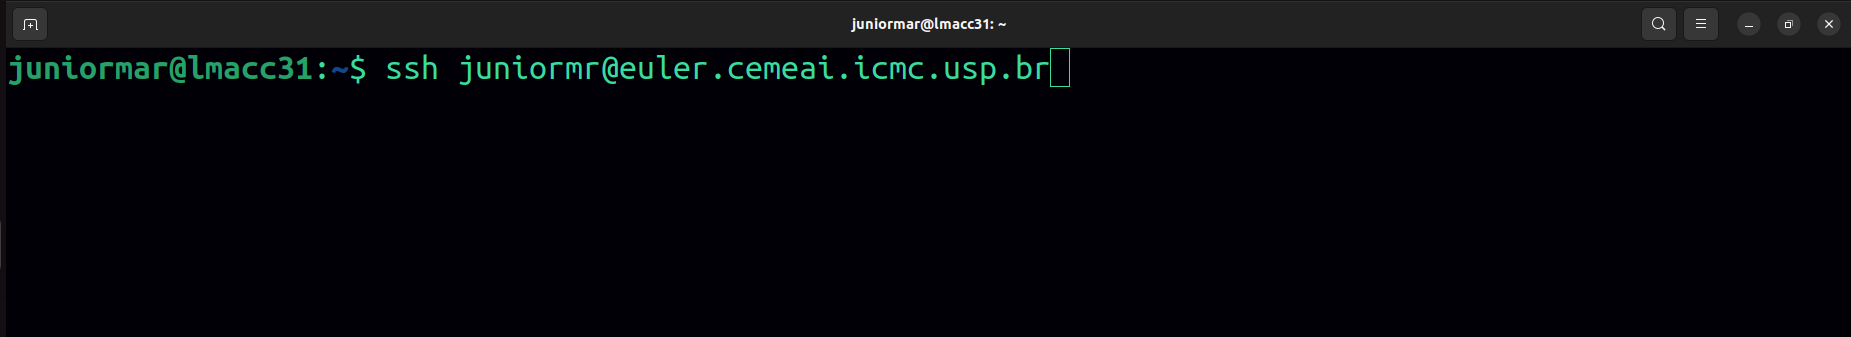
\includegraphics[trim = 0mm 60mm 190mm 0mm,clip,width=1.05\linewidth]{figures/login_euler.png}
		\label{fig:logineuler}
	\end{figure}
    \item[] Após digitar as senhas, deverá aparecer a tela inicial do Euler
    \begin{figure}[htb]
    	\centering
    	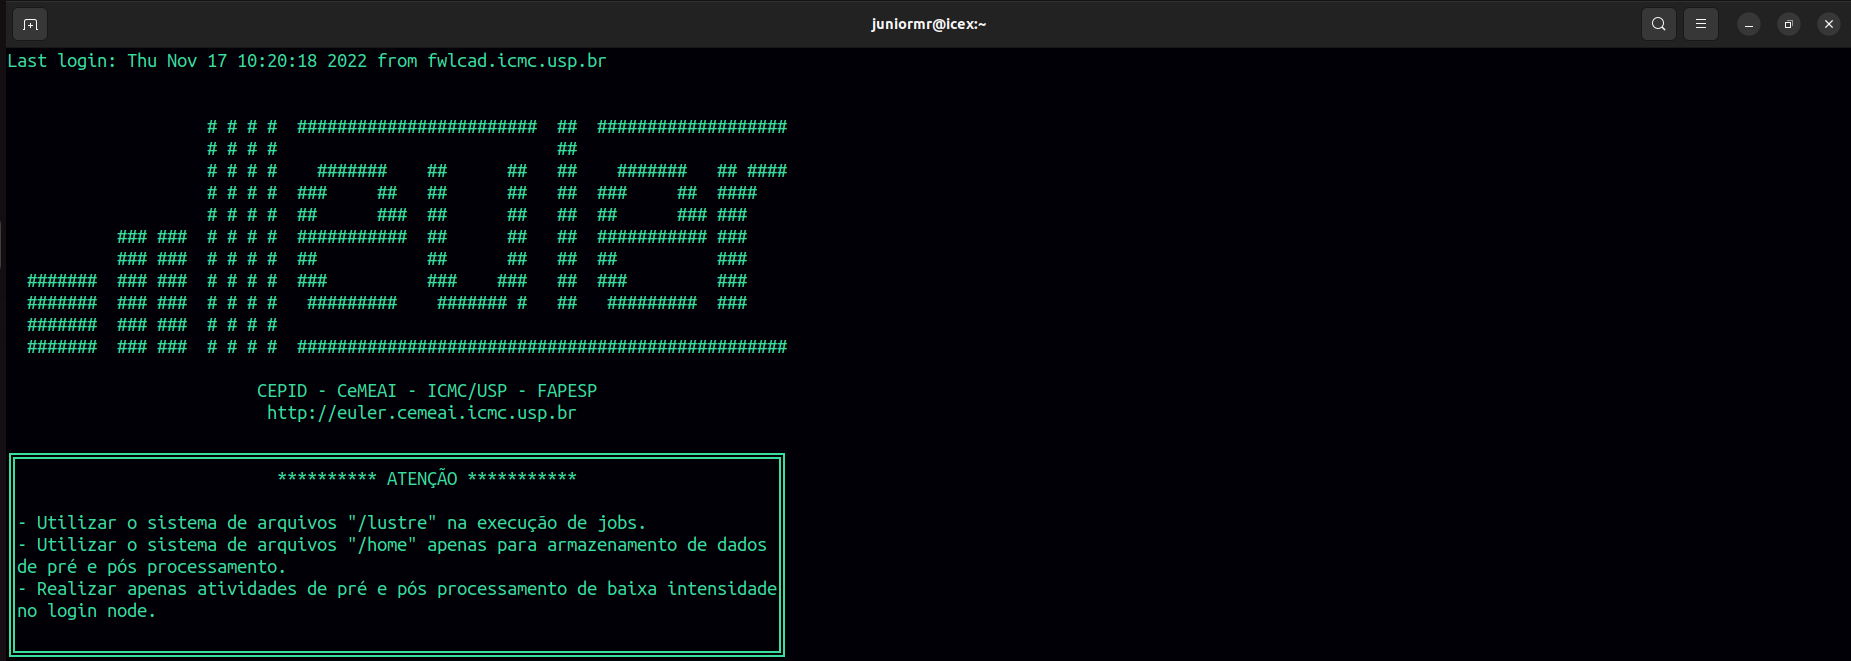
\includegraphics[trim = 0mm 0mm 190mm 0mm,clip,width=1.05\linewidth]{figures/login_euler_2.png}
    	\label{fig:logineuler2}
    \end{figure}
	\item \textbf{\colorbox{red}{Observação importante!!!}} Neste ponto de acesso ao cluster faz-se necessário alertar da correta utilização dos ambientes ``home'' e ``lustre'' do Cluster Euler. Para uma boa utilização de todos os usuários, recomenda-se \textbf{\textcolor{red}{NUNCA}} rodar um código ou simular algo diretamente nos nós de login, para isso, deve-se fazer a submissão dos trabalhos para os nós de simulação por meio de um arquivo com extensão \textbf{\textit{.job}}. O ambiente home tem como finalidade principal o armazenamento de dados e, o ambiente lustre, é destinado para a submissão das simulações. Para tal, faça o que segue:
	\item \textbf{cd /lustre/usuario} := Muda do diretório ``home'' para o ``lustre'' do usuário.\\ \textbf{\underline{Exemplo:}}
	\begin{figure}[htb]
		\centering
		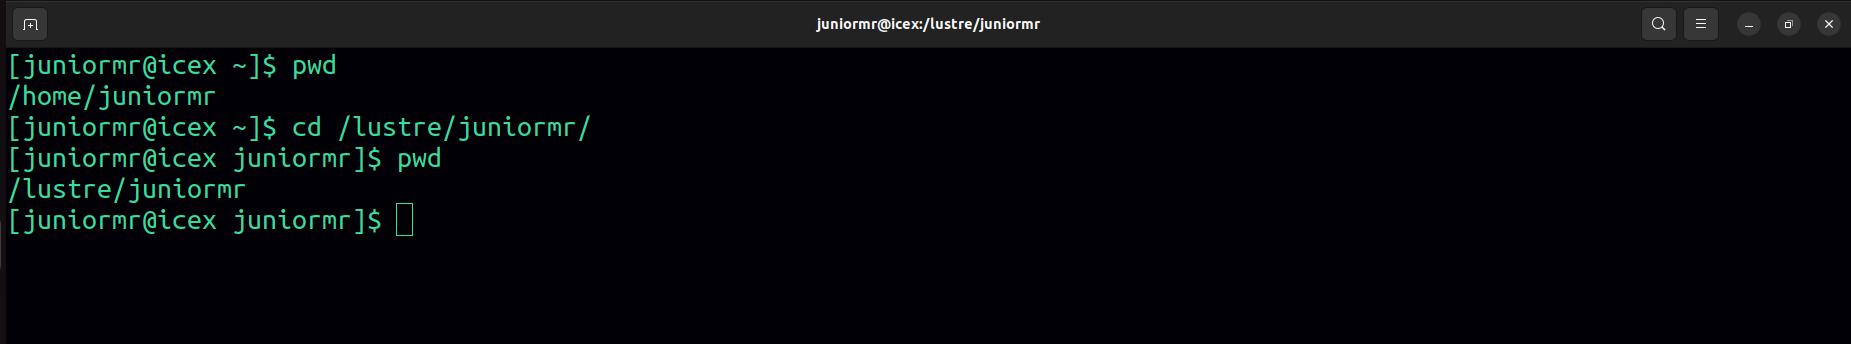
\includegraphics[trim = 0mm 20mm 190mm 0mm,clip,width=1.05\linewidth]{figures/mudar_para_lustre.png}
		\label{fig:muda_lustre}
	\end{figure}	
	
	\item Para copiar um diretório da sua máquina para o cluster deve-se inicialmente abrir um terminar no diretório do que se deseja enviar para o cluster (diretório ou arquivo) e utilizar o seguinte comando:
	
	\hspace{-1.7cm}
	\textbf{scp -r nome\_do\_diretorio usuario@euler.cemeai.icmc.usp.br:/diretorio\_de\_destino\_no\_cluster/}
	
	\textbf{\underline{Exemplo:}}
    \begin{figure}[htb]
    	\centering
    	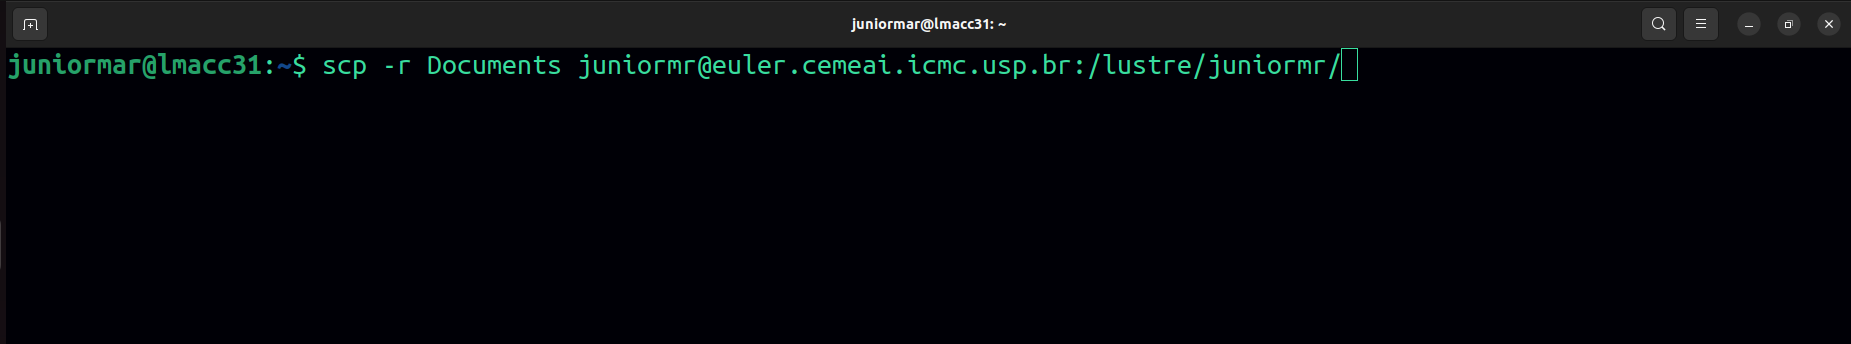
\includegraphics[trim = 0mm 70mm 160mm 0mm,clip,width=1.05\linewidth]{figures/send.png}
    	\label{fig:send}
    \end{figure}
	\item Para copiar/baixar um diretório ou arquivo do cluster para sua máquina deve-se inicialmente abrir um terminar no diretório ao qual se deseja baixar o arquivo ou o diretório que estão no cluster e utilizar o seguinte comando:
	
	\hspace{-1.7cm}
	\textbf{scp -r usuario@euler.cemeai.icmc.usp.br:/local\_do\_arquivo/nome\_do\_diretorio local\_de\_destino/$\mbox{  .}$}
	
	\textbf{\underline{Exemplo:}}
	\begin{figure}[htb]
		\centering
		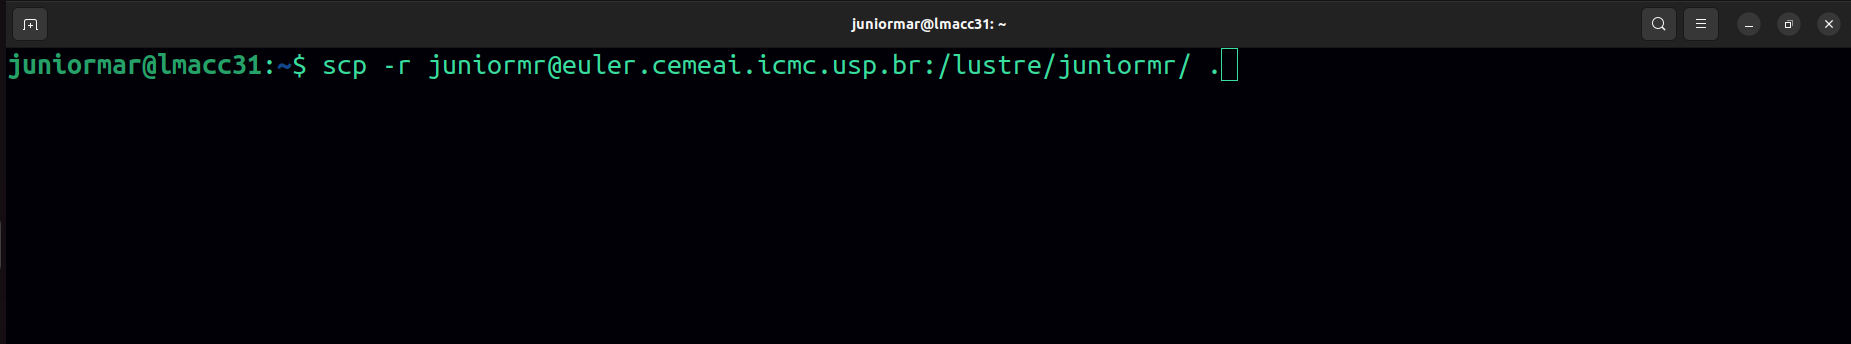
\includegraphics[trim = 0mm 70mm 190mm 0mm,clip,width=1.05\linewidth]{figures/download.png}
		\label{fig:recive}
	\end{figure}
	
	\item Para conseguir executar o código no cluster é necessário submeter o código. Para isso, é necessário o uso de um arquivo de submissão com a extensão \textbf{\textit{.job}}, como apresentado no exemplo da figura abaixo:
	\begin{figure}[htb]
		\centering
		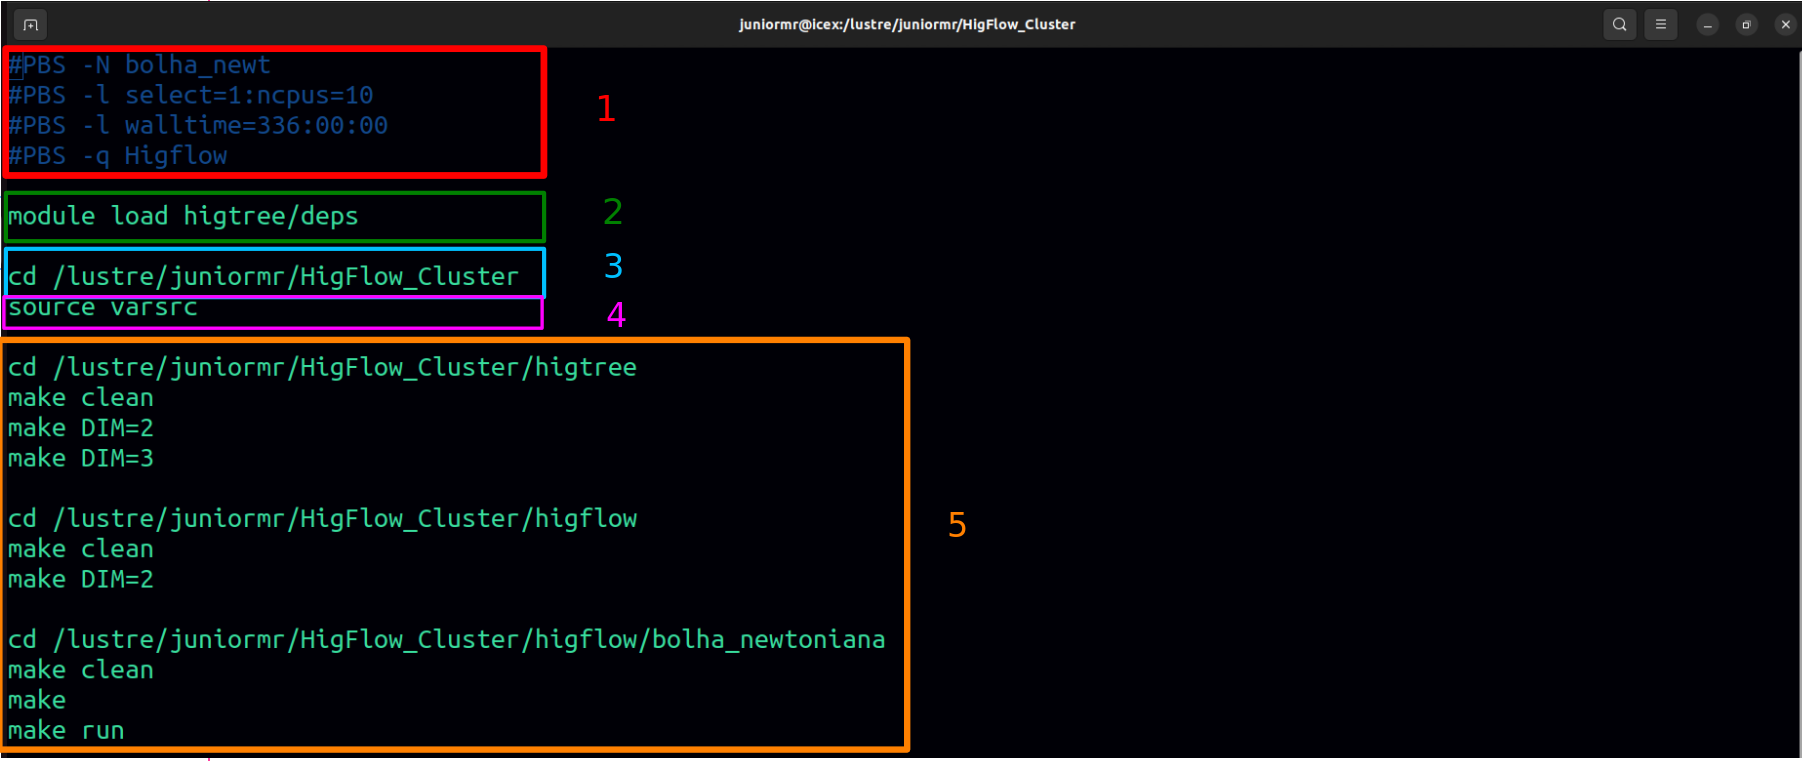
\includegraphics[trim = 0mm 0mm 210mm 0mm,clip,width=1.05\linewidth]{figures/job_box.png}
		\label{fig:job}
	\end{figure}
	\begin{enumerate}
		\item Cabeçalho: 
			\subitem $\textbf{\#PBS\ -N\ bolha\_newt}$: Dá o nome ``bolha\_newt'' ao trabalho na fila dos trabalhos no cluster;
			\subitem $\textbf{\#PBS\ -l\ select=1:ncpus=10}$: Seleciona o número de nós e de `cpus' que devem ser utilizados (neste caso foram 10 processadores/cpus);
			\subitem $\textbf{\#PBS\ -l\ walltime=336:00:00}$: Seleciona o tempo estimado de simulação (depois do termino do tempo estipulado, a simulação é interrompida);
			\subitem $\textbf{\#PBS\ -q\ Higflow}$: Coloca a submissão em uma fila especial do cluster (denominada ``Higflow''). Atualmente é necessário que se peça ao técnico responsável que se adicione a essa fila especial para que se consiga executar teste do projeto no cluster;
		\item Módulos a serem carregados para compilação e execução das simulações (neste caso carrega todas as dependências necessárias para executar o projeto atual que está no GitHub no cluster);
		\item Localização do arquivo para submissão;
		\item O arquivo ``varsrc'' disponível no projeto dispensa a necessidade de se alterar o arquivo ``.bashrc'' que era necessário antigamente. Para esse arquivo deve tomar um cuidado especial com o caminho destinado para o Petsc. No caso do Cluster Euler esse caminho, que está definido no aquivo, não é necessário e portanto deve-se editar o arquivo retirando esse caminho do arquivo ``varsrc'';
		\item Comando para compilar e executar o código no cluster (como já é feito normalmente);
		\item \textbf{qsub nome\_do\_arquivo.job}: Utilizado para submissão de um trabalho.
	\end{enumerate}
\end{itemize}

\section{HigFlow no Cluster - Passos iniciais}\label{sec:clu_pas_ini}

Para que consiga utilizar o cluster para realizar os testes do HigFlow, inicialmente deve-se criar uma conta pelo do site \href{http://www.cemeai.icmc.usp.br/Euler/index.html}{site do Cluster}( Manual para uso do cluster - \href{http://resources.altair.com/pbs/documentation/support/PBSProUserGuide12.2.pdf}{manual}). Para enviar o código para cluster, deve inicialmente criar uma pasta no cluster onde será armazenado o código. Para o envio existem duas possibilidades
\begin{itemize}
	\item \textbf{git clone https://github.com/antoniocastelofilho/HigFlow.git} $:=$ faz uma cópia do código armazenado no GitHub. Para esse caso, deve-se ter acesso ao projeto no GitHub
	\item \textbf{scp -r diretorio usuario@euler.cemeai.icmc.usp.br:/diretorio\_de\_destino\_no\_cluster/}	$:=$ Envia o ``diretorio" (com o código do HigFlow) para o cluster Euler para o ``diretorio\_de\_destino\_no\_cluster"
\end{itemize}
 
 Após o envio do código, deve-se alterar o arquivo ``bashrc" do cluster seguindo os passos abaixo:
 \begin{itemize}
 	\item \textbf{vi $\sim$/.bashrc} $:=$ Abre o arquivo ``bashrc" para ser editado pelo \textbf{vi};
 	\item Acrescente as linhas a seguir no arquivo ``bashrc":\\
 	\textbf{export HIGTREE\_DIR=/diretorio\_do\_higflow\_no\_cluster/higtree}\\
 	\textbf{export HIGFLOW\_DIR=/diretorio\_do\_higflow\_no\_cluster/higflow}\\
 	
 	\textbf{Exemplo:} Como exemplo, no usuário ``juniormr" fez-se o download do código no diretório ``/lustre/juniormr/HigFlow", assim as linhas adicionadas serão\\
 	\begin{figure}[htb]
 		\centering
 		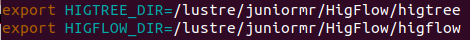
\includegraphics[width=0.98\linewidth]{figures/export_bashrc}
 		\label{fig:fig01}
 	\end{figure}
 \end{itemize}

\section{Modulo ``higtree/deps" para o sistema HigFlow no cluster}

Para conseguir compilar o código no cluster é necessário carregar o modulo ``higtree/deps", fazendo
\begin{itemize}
	\item \textbf{module load higtree/deps} $:=$ Comando que carrega os módulos necessários para compilar;
	\item \textbf{module list} $:=$ Comando para mostrar os módulos carregados. Quando carregado o modulo ``higtree/deps", ao digitar ``module list" tem-se
	\begin{figure}[htb]
		\centering
		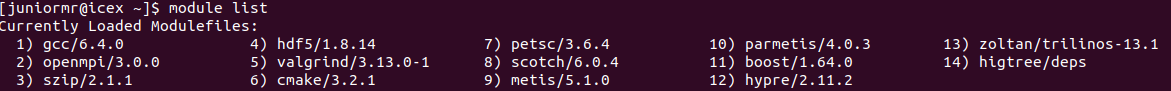
\includegraphics[width=1.0\linewidth]{figures/module_list}
		\label{fig:fig02}
	\end{figure}
\end{itemize}

\section{Job}\label{sec:job_fun}

Para rodar os teste é necessário criar um arquivo ``.job" para submeter ao cluster. Abaixo segue um exemplo
\begin{figure}[htb]
	\centering
	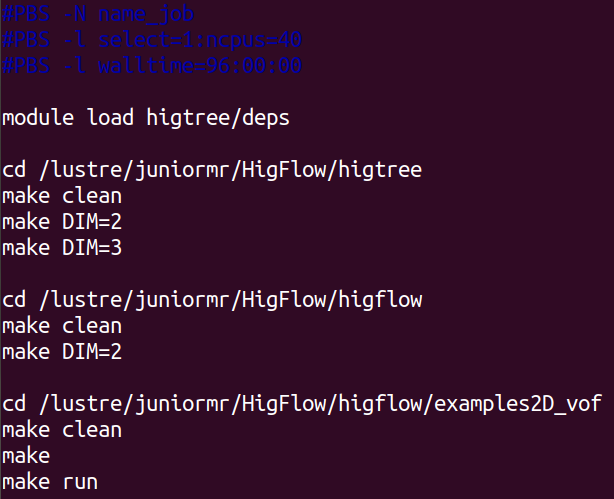
\includegraphics[width=0.80\linewidth]{figures/submission_job}
	\label{fig:fig03}
\end{figure}


%\bibliographystyle{plain}
%\bibliography{cluster_euler}

\end{document}
